The CMA-ES source code handles box constraints natively using the "repair and penalize" procedure. This consists in repairing non-feasible sampled points before inputing them to the model; and penalizing (i.e. increasing the value of the fitness function) proportionally to the distance between the unfeasible point and the feasible space. This method forces the algorithm to eventually enter and stay in the feasible domain while avoiding evaluating non-allowed points.\\
However, the source code does not handle linear constraints. We describe here how we apply manually this repair \& penalize procedure to reflect the two linear constraints shown in \ref{subsec:statement}.\\
\\
%
%For the multiple-knob groups, the boundaries are refined using the same idea as in \ref{subsec:single} applied to the \emph{knob group flow demands}. The CMA-ES code requires however to implement ourselves a repair \& penalize process instead of changing the knob boundaries, as the constraints will not be box but linear. \color{red}(<- rephrase this)\color{black}.\\
%\\
%For each multiple-knob group, we want to impose that the total flow brought by the knobs is in a range based on its \emph{flow demand} and computed similarly to \ref{subsec:single}.\\
%The implementation is done by leaving the knob boundaries to their physical value (see \ref{subsec:naive}) but \emph{repairing} the points sampled by CMA-ES before imputing them to the simulator.\\
%This reparation consists in a projection of the sampled point to the closest point on the feasible space, which is the intersection of the hypercube formed by the physical constraints and the volume between the two hyperplans defined by the range of the flow demands.\color{red}(<- rewrite this)\color{black}\\
%\\
\emph{Repairing:}\\
\\
Let $\underline{\vec{k}}^{(p)}$ the knobs vector sampled by CMA-ES at iteration p (i.e. before repairment).\\
%Let $J=\{j\in \llbracket 1,\gamma \rrbracket\ |\ Card(g_{j}>1)\}$\\
%\\
%$\forall j\in J,\ \Delta_{j}^{min}=\min{\{\lambda.\Delta_{j};\Delta_{j}-I^{local}\}}$\\
%$\ and\ \Delta_{j}^{max}=\max{\{\Lambda.\Delta_{j};\Delta_{j}+I^{local}\}}$\\
The projection is implemented using the following program in a standard quadratic optimization solver:\\
\\
$minimize \ \ \ \ \ \ \norm{\vec{k}^{(p)}-\underline{\vec{k}}^{(p)}}_{2}$\\
$s.t.\ \ \ \forall i\in{G}, \ \ \Delta_{i}^{-}< \sum_{j\in{g_{i}}} \sigma_{j}.k_{j}.\Theta<\Delta_{i}^{+}$\\
$and\ \widetilde{VMT}^{-}\leq\mathlarger{\sum\limits_{i\in K}}\biggl[\sigma_{i}.k_{i}.\Theta.	\sum\limits_{\underset{j>i}{j\in T}}L_{j}\biggr]+VMT^{ref}\leq \widetilde{VMT}^{+}\nonumber $\\
$and\ \ \ \ \vec{k}^{(p)}\in \mathscr{B}$\\
\\
Let us illustrate the effect of this program with an example. We suppose that the $\widetilde{TVM}^{\pm}$ condition above is enough loose for the condition to be respected without influencing the projection (often verified in practice).
\begin{figure}[h!]
\centering
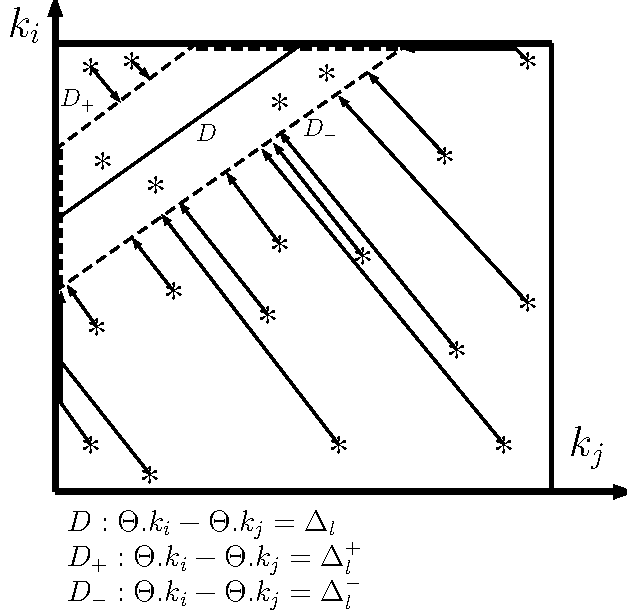
\includegraphics[width=3in]{figures/proj.pdf}
\caption{Example of projection on a two-knobs group}
\label{fig:proj}
\end{figure}
Fig. \ref{fig:proj} above displays, for a two-knobs group $g_{l}=\{i,j\}$, the projection of several sampled points due to the two remaining conditions ($\Delta_{l}^{\pm}$ and $\mathscr{B}$). $D$ is the hyper-plan (straight line in dimension 2) on which the knob group flow will have the exact value $\Delta_{l}$.
The two \emph{tolerance hyper-plans} on which the knob group flow value will be $\Delta_{l}^{+}$ and $\Delta_{l}^{-}$ are respectively $D^{+}$ and $D^{-}$.
In addition, the external square is the hyper-cube corresponding to the physical boundaries of the two knobs. 
The points sampled in the feasible space (inside the doted line trapezium) remain untouched while the others are projected on the nearest point of the edge of the feasible space.\\
This repair ensures that only feasible values of the input are tested and that the algorithm will not get stuck in an unfeasible well of the physical boundaries hyper-cube.\\

\emph{Penalizing:}\\
\\
At each evaluation, a penalization proportional to the distance between the projected and original point is added to the fitness function. This ensures that the algorithm will come closer to the feasible space at every iteration until eventually entering and staying inside it. This feature is important as it avoids two imbalances on the sampling:
\begin{itemize}
	\item Testing more points on the edges than we should: if the algorithm is left sampling points far from the edges, without penalization, it will have no incentive to prefer sampling next to the feasible space than far. This is an obstacle from entering the feasible space, as all the points on the straight lines perpendicular to the edges would be equivalent. This would lead to a situation where it is common that too much (or all) of the points are sampled on the edges, CMA-ES converging far from the feasible space.\color{red}(<- rewrite this)\color{black}.
	\item Imbalance between the edge points tested: the edge points which are the projection of more unfeasible hyper-cube points than others will be sampled unfairly more often.\\
	\emph{Example:} in Fig. \ref{fig:proj}, the points on the mediator of the segment formed by the intersections of D and the square while inside the square are more numerous than the points on any other straight with same slope.\\
The points on one of these straights and below the feasible space are all projected to the same point of the edge of the feasible space. Therefore, without penalization, the middle of the segment cited above would be sampled more often than the other points of its edge, for a reason that is not the simulation output it leads to. 
\end{itemize}

The penalization is normalized by a factor which is the distance between the physical maximums and minimums vectors, reflecting the \emph{order of magnitude} of the search space.
\begin{equation*}
	E_{proj}(\underline{\vec{k}}^{(p)},\vec{k}^{(p)})=\frac{\norm{\vec{k}^{(p)}-\underline{\vec{k}}^{(p)}}_{2}}{\norm{\begin{bmatrix}m_{1}\\m_{2}\\\vdots\\m_{\kappa}\end{bmatrix}-\begin{bmatrix}0\\0\\\vdots\\0\end{bmatrix}}_{2}}
\end{equation*}
A fourth contribution $w_{4}.E_{proj}(\underline{\vec{k}}^{(p)},\vec{k}^{(p)})$ is therefore added to the fitness function.\\
\\
With the same definitions as in \ref{subsec:fitnessintro} and\\
$\sum_{i=1}^{4} w_{i}=1\ and\ \forall i\in\llbracket 1,4\rrbracket\ w_{i}\geq 0$,\\
\\
the final fitness function used is $J$ defined by :\\
\begin{equation*}
		J:
		\left|
  		\begin{array}{rcl}
    	\mathscr{B} & \longrightarrow &[0,100] \\
    	\underline{\vec{k}}^{(p)} & \longmapsto &  \Phi(\vec{k}^{(p)})+w_{4}.E_{proj}(\underline{\vec{k}}^{(p)},\vec{k}^{(p)}) \\
  	\end{array}
	\right.
\end{equation*}
\\
We denote $J^{*}$ the minimum of $J$ encountered by CMA-ES during its search :
\begin{equation*}
	J^{*}=\min_{p}{J({\vec{k}^{(p)})}}
\end{equation*}
\\
\emph{Single-knob group specificity:} For a single-knob group, the condition Eq. \ref{eq:ineq} is equivalent to hard boundaries for the concerned knob (one equation in one dimension). In this case, the projection due to Eq. \ref{eq:ineq} is not implemented but the physical boundaries (from $\mathscr{B}$) of the knob input to CMA-ES are replaced by these new boundaries, if they are narrower :\\
\\
$\forall\ i\in G\ s.t.\ Card(g_{i})=1,\ i.e.\ g_{i}=\{j\}\ :$
\begin{equation}
	\frac{\max{\big\{0;|\Delta_{i}^{-}|\big\}}}{\Theta}\leq k_{j} \leq \frac{\min{\big\{m_{i};|\Delta_{i}^{+}|\big\}}}{\Theta}
\end{equation}
